\documentclass{article}
\usepackage{graphicx} % Required for inserting images
\usepackage{amssymb}
\usepackage{amsmath}
\usepackage{lipsum}
\title{\textbf{k-NEAREST NEIGHBOURS}\\EPOCH IIT HYDERABAD}
\author{Rishitha Pallala }
\date{18 August 2023}

\begin{document}

\maketitle
\section{Introduction}
 k-Nearest Neighbours is a supervised machine learning algorithm. It is usually used for classification .Although, it works for regression also. This model assigns the label to new data points, by checking and averaging the labels of k-nearest neighbours . The nearness is determined by the distance of the points from the new point.  \\\\
 For classification: the label is assigned as the label of majority of nearest neighbours\\
 For regression: the label assigned is the mean or median of the k nearest neighbours.
 \section{ Optimal K}
 The value of K determines the quality of our model. The two parameters are training error rate and validation error rate.
 the training error for k=1 is 0 , and increases as we increase the k value.\\\\
 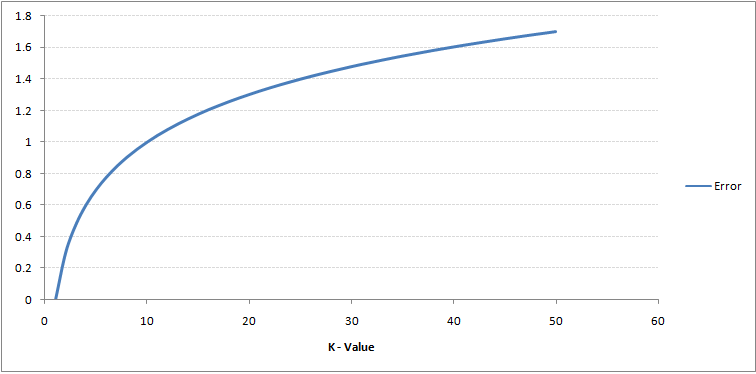
\includegraphics[scale=0.4]{training-error.png}\\\\
 The validation error rate os high for k=1, due to overfitting the curve reaches the minima and then increases for increasing k-value.\\\\
 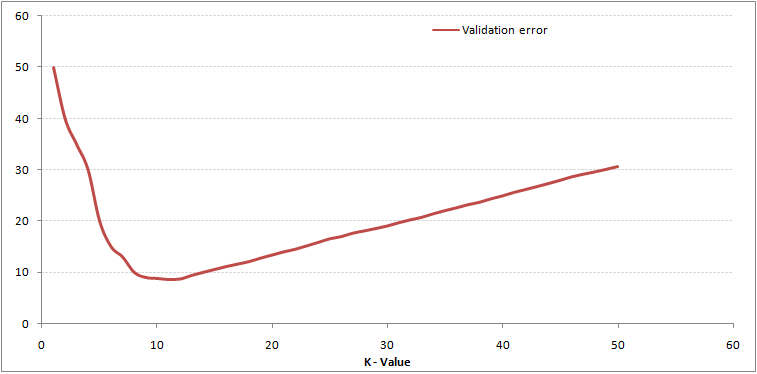
\includegraphics[scale=0.4]{validation-error_11.png}\\\\
 we can take the k with minimum error as the optimal k.Hence , this model is intuitive and is used for predictions due to less calculation time. 
\end{document}